\section{Methodology}
\label{sec:metho}
In this section, we describle the generation of PGT and proposed video-based semantic segmentation network.
%
We first introduce generation steps of PGT, and then present the overview of video-based semantic segmentation network.

{\bf Pseudo Ground Truth Generation.}
%
Given the ground truth labeling ${G_t}$ of a frame ${F_t}$ in the training set, the semantic labels ${G_t}$ propogate to its adjacent frames via two steps.
%
First, the method of image transformation is applied to generate rough PGT by setting thresholds of homograph matrix ${H}$ as well as controlling propagation range ${P_r}$.
%
To ensure the quality of generated PGT, the thresholds of homograph matrix are set as follows while the ${P_r}$ is set to 10.

\begin{equation}
\centering
\begin{aligned}
H
=
\left[
\begin{array}{ccc}
h_{00} & h_{01} & h_{02}\\
h_{10} & h_{11} & h_{12}\\
h_{20} & h_{21} & h_{22}\\
\end{array}
\right] \\
0.95<\max{\left\{h_{00},h_{01},h_{10},h_{11}\right\}}&<1.05\\
\max{\left\{h_{02},h_{12},h_{20},h_{21},h_{22}\right\}}&<15\\
\end{aligned}
\end{equation}

Second, filtering label manually once and deleting labels with excessive noise.
%
Comparing with dense image annotation, filttering PGT took about half a day (2-3sec/image) for a human.
%
We believe that performance boost received at the cost of a small amount of manpower is valuable.
%
To this end, the total number of PGT frames obtained is 7626.
%
Although PGT includes noise samples, the diversity of training set are also enriched. 


{\bf Video-based Semantic Segmentation Network.}
%
Fig.~\ref{fig:Pipeline} illustrates the overall architecture of our proposed video-based semantic segmentation network, which mainly consist of three parts: the basic segmentation network, the warp operation between frames, and the supervision module.
%
First, the current frame is passed through the basic segmentation network to generate prediction.
%
Meanwhile, the warp operation is used to warp the previous frame prediction to align with current frame by optical flow.
%
And then, the warped previous frame prediction plays a role of a supervisory item of supervision module to constrain the consistency of prediction results of neighboring image frames.
%
Finally, the PGT of current frame as the other supervisory item of supervision module is introduced to guarantee that the prediction results are as accurate as possible.



The basic segmentation network could employ any existing network structures. 
%
To obtain better segmentation result, we use RDFNet\cite{Park2017} that is a high-precision network for scene parsing as our basic segmentation netwrok. 
%
The input of RDFNet is RGBD data. 
%
The depthmap is encoded into a 3D image called HHA which encodes height above ground and angle with gravity for each pixel in addition to the horizontal disparity.
%
Four multi-modal feature fusions (MMF) are used to fully exploit multi-level HHA and RGB images features.
%
And then four RefineNet blocks are applied to refine the output of MMF gradually.
%
More details of RDFNet could be found in \cite{Park2017}. 
%
And the network structure of RDFNet is reviewed in Fig.~\ref{fig:Pipeline}.

In our warp operation, the optical flow is calculated by PWC-Net \cite{Sun2018} that is a highly efficient and accurate model.
%
Please refer to \cite{Sun2018} for more details.
%
After getting optical flow, the score map of previous frame ${S_{t-1}}$ is warped to align with the current frame:
\begin{equation}
\centering
\hat{S}_{t-1}=Warp(S_{t-1},O_t)
\end{equation}
where ${\hat{S}_{t-1}}$ denotes the warped score map of previous frame, and ${O_t}$ is the dense correspndence field. 
%
In our work, we implement ${Warp}$ as a bilinear interpolation of $S_{t-1}$.
%
And adding a Argmax layer to extract the warped prediction of previous frame.
\begin{equation}
\centering
W_{t-1}=Argmax(\hat{S}_{t-1})
\end{equation}

Two supervisory items constitute our supervision module.
%
One is to monitor the prediction result of the current frame to be consistent with the PGT.
%
The other is for constraining consistency of prediction results between frames by an additional loss function called consistentency loss. 
%
To leverage two items of supervision module, we propose a trust parameter ${\lambda}$ for weighing two losses. 
%
In addition, the trust parameter ${\lambda}$ is also used to represent what kind of supervisory item the model trust in.
%
Our total loss function is defined as follows.
\begin{equation}
\centering
\begin{aligned}
L_{All}= \lambda L_{PGT} +(1-\lambda)L_{Consistency}
\end{aligned}
\end{equation}

\begin{figure}[htpb]
	\centering
	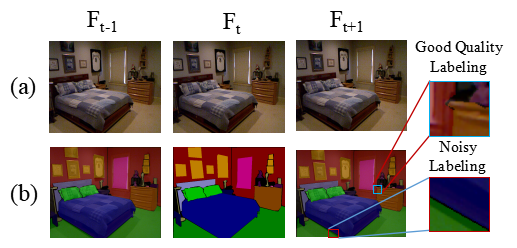
\includegraphics[scale=0.65]{figure/PGT.png}
	\caption{Qualitative results of our PGT. (a) is a sequence of images. And the right side shows details of good quality pseudo labels and noisy pseuso labels respectively. }
	\label{fig:PGT}
\end{figure}

Here, ${L_{PGT}}$ means the loss comes from first supervision item.
%
${L_{Consistency}}$ denotes the loss from second supervision item which constrains the predicted results are consistent in time dimension. 
%
Both ${L_{PGT}}$ and ${L_{Consistency}}$ are softmax loss, as described below.
\begin{equation}
{\setlength\abovedisplayskip{8pt}
	\setlength\belowdisplayskip{-8pt}
\centering
\begin{aligned}
L_{PGT} = -&\sum_{i=0}^Il(\vec p_i,\vec y_i) \\
L_{Consistency} &= -\sum_{i=0}^Il(\vec w_i,\vec y_i)\\
l(\vec p_i,\vec y_i) = -&\sum_{k=0}^c \,p_{ik}\log{y_{ik}}\;,\; \vec y_{i} = f(x_{i})\\
\end{aligned}
}
\end{equation}

Here ${x_i}$ and ${\vec y_i}$ denote a pixel of input and the corresponding output of semantic segmentation model respectively. 
%
${c}$ represents number of categories, and ${I}$ is the number of pixels in the RGB image. 
%
${\vec p_i}$ and ${\vec w_i}$ are an one-hot vector for each pixel of PGT and warped previous frame prediction respectively. 
%
${l(\cdot)}$ is softmax loss of one pixel, and ${f(\cdot)}$ is our basic segmentation network. 
%
By these two losses, we can constrain the accuracy and consistency of prediction result simultaneously.
